\documentclass{../presentation}

\title{Τριγωνομετρία}
\subtitle{Τριγωνομετρικοί Αριθμοί - Ακτίνια - Τριγωνομετρικός Κύκλος}
\author[Λόλας]{Κωνσταντίνος Λόλας}
\date{}

\begin{document}

\begin{frame}
  \titlepage
\end{frame}

\section{Θεωρία}
\begin{frame}{Απλή εφαρμογή ακτινίων}
  \begin{itemize}
    \item<1-> Τι είναι το 1 ακτίνιο?
    \item<2-> Τι είναι τα 2 ακτίνια?
    \item<3-> Τι είναι τα 4.1 ακτίνια?
    \item<4-> Τι είναι τα $α$ ακτίνια?
  \end{itemize}
  \begin{block}{Μήκος Τοξου}<5->
    Το τόξο $α$ ακτινίων ενός κύκλου ακτίνας $ρ$ έχει μήκος
    $$S=αρ$$
  \end{block}
  \onslide<6-> Άσκηση 3 σχολικού
\end{frame}

\section{Ασκήσεις}

\begin{askisi}
  Να υπολογίσετε τους τριγωνομετρικούς αριθμούς της γωνίας $ω$ που φαίνεται στο σχήμα

  \centering
  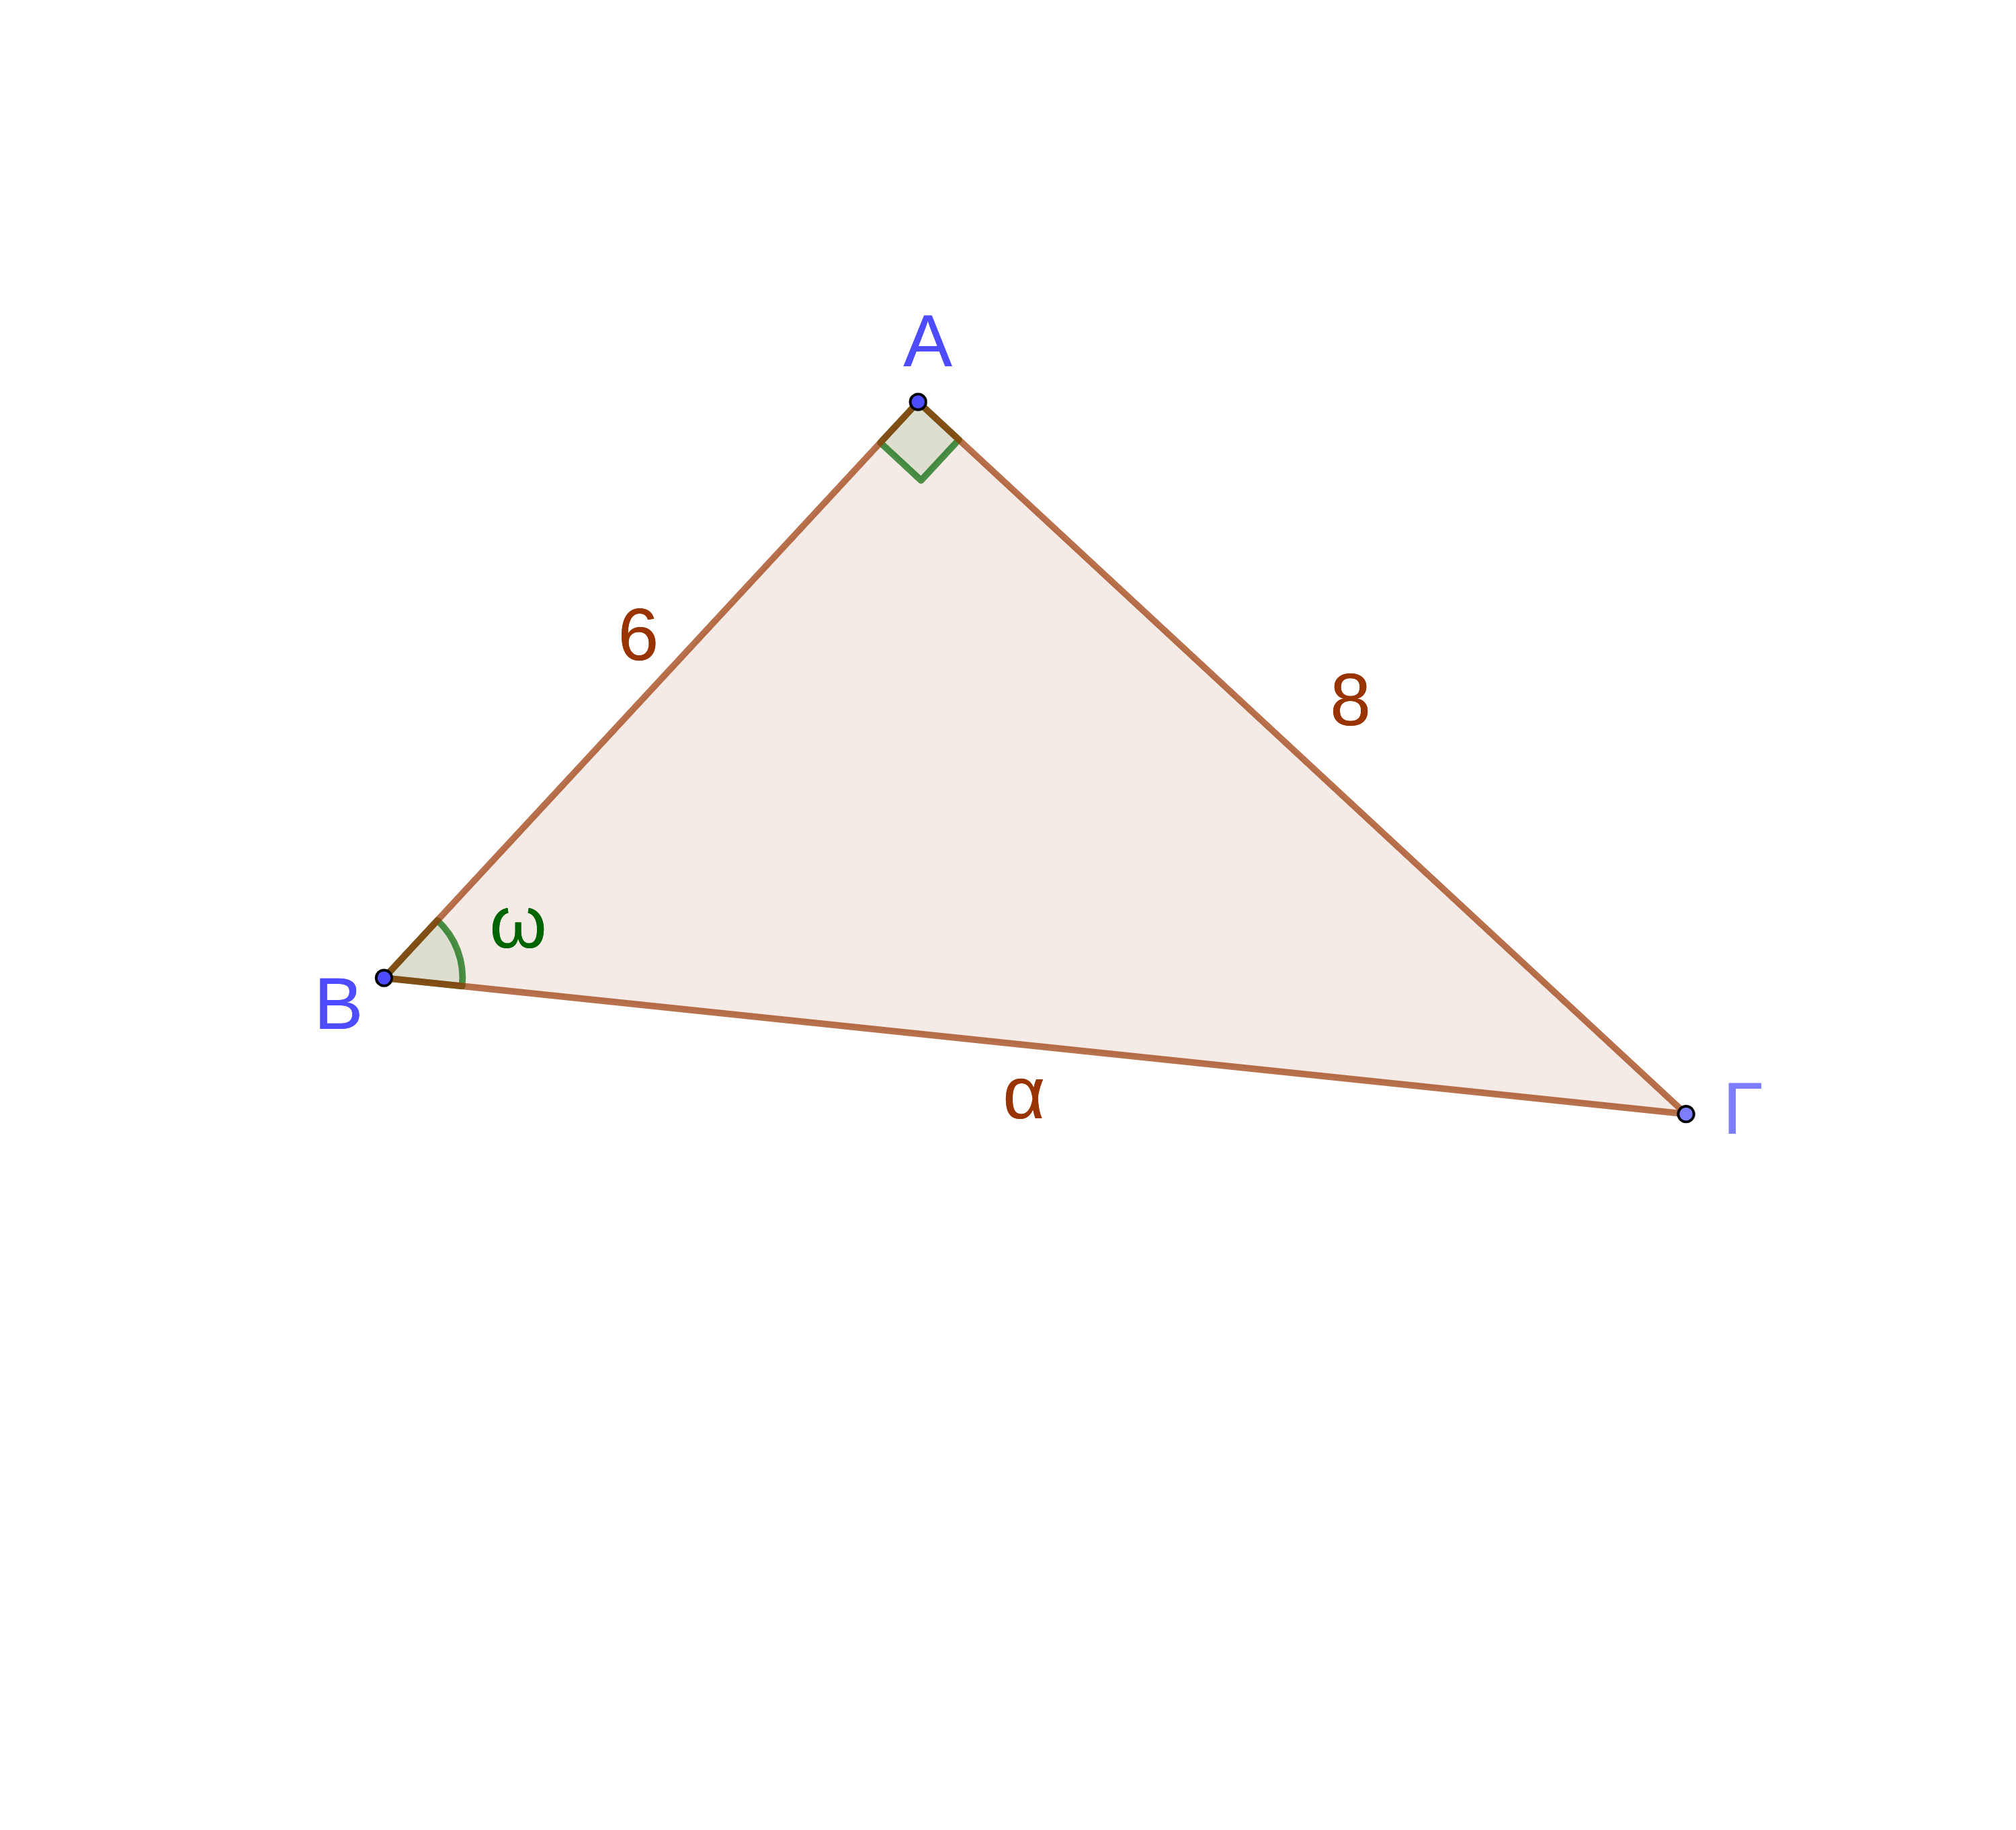
\includegraphics[width=0.8\textwidth]{"./images/3.1.1_1.png"}
\end{askisi}

\begin{askisi}
  Στο σχήμα είναι $συνω=\dfrac{8}{17}$. Να βρείτε το $x$ και την $εφω$

  \centering
  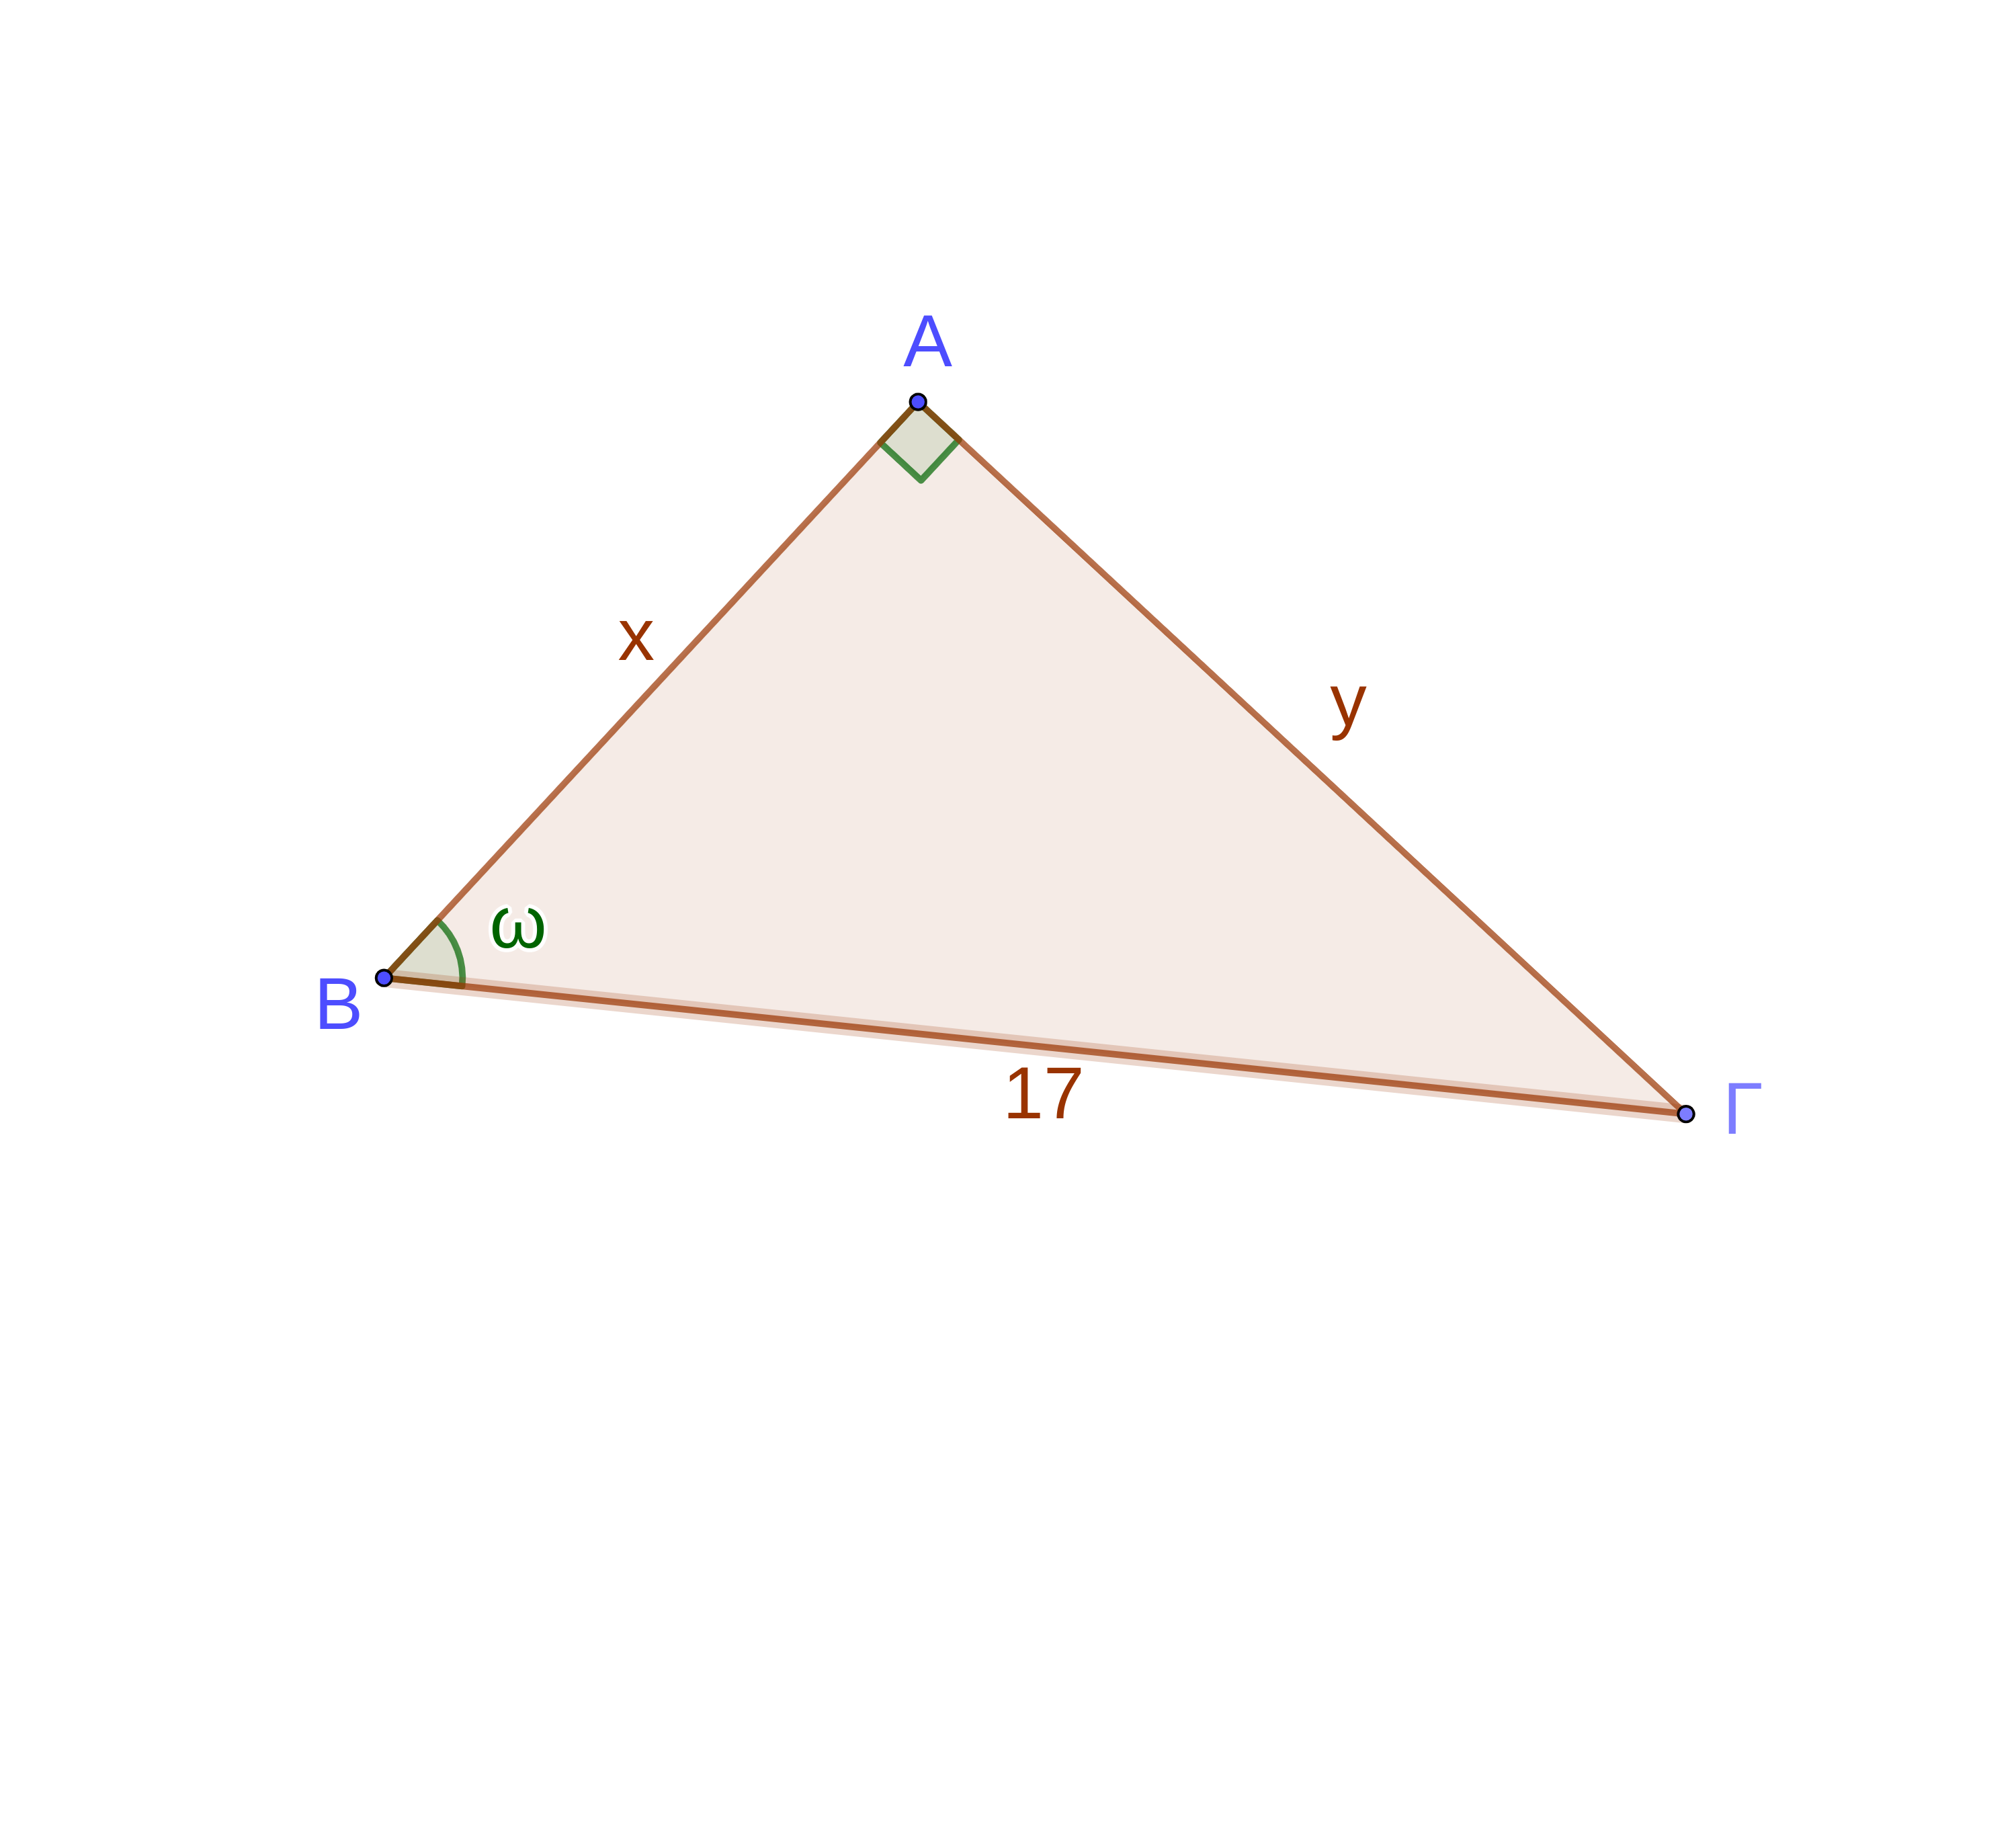
\includegraphics[width=0.6\textwidth]{"./images/3.1.1_2.png"}
\end{askisi}

\begin{askisi}
  Στο σχήμα, να υπολογίσετε τα $x$ και $y$. Δίνονται $συν20^{\circ}=0.94$, $ημ20^{\circ}=0.34$ και $συν36^{\circ}=0.81$

  \centering
  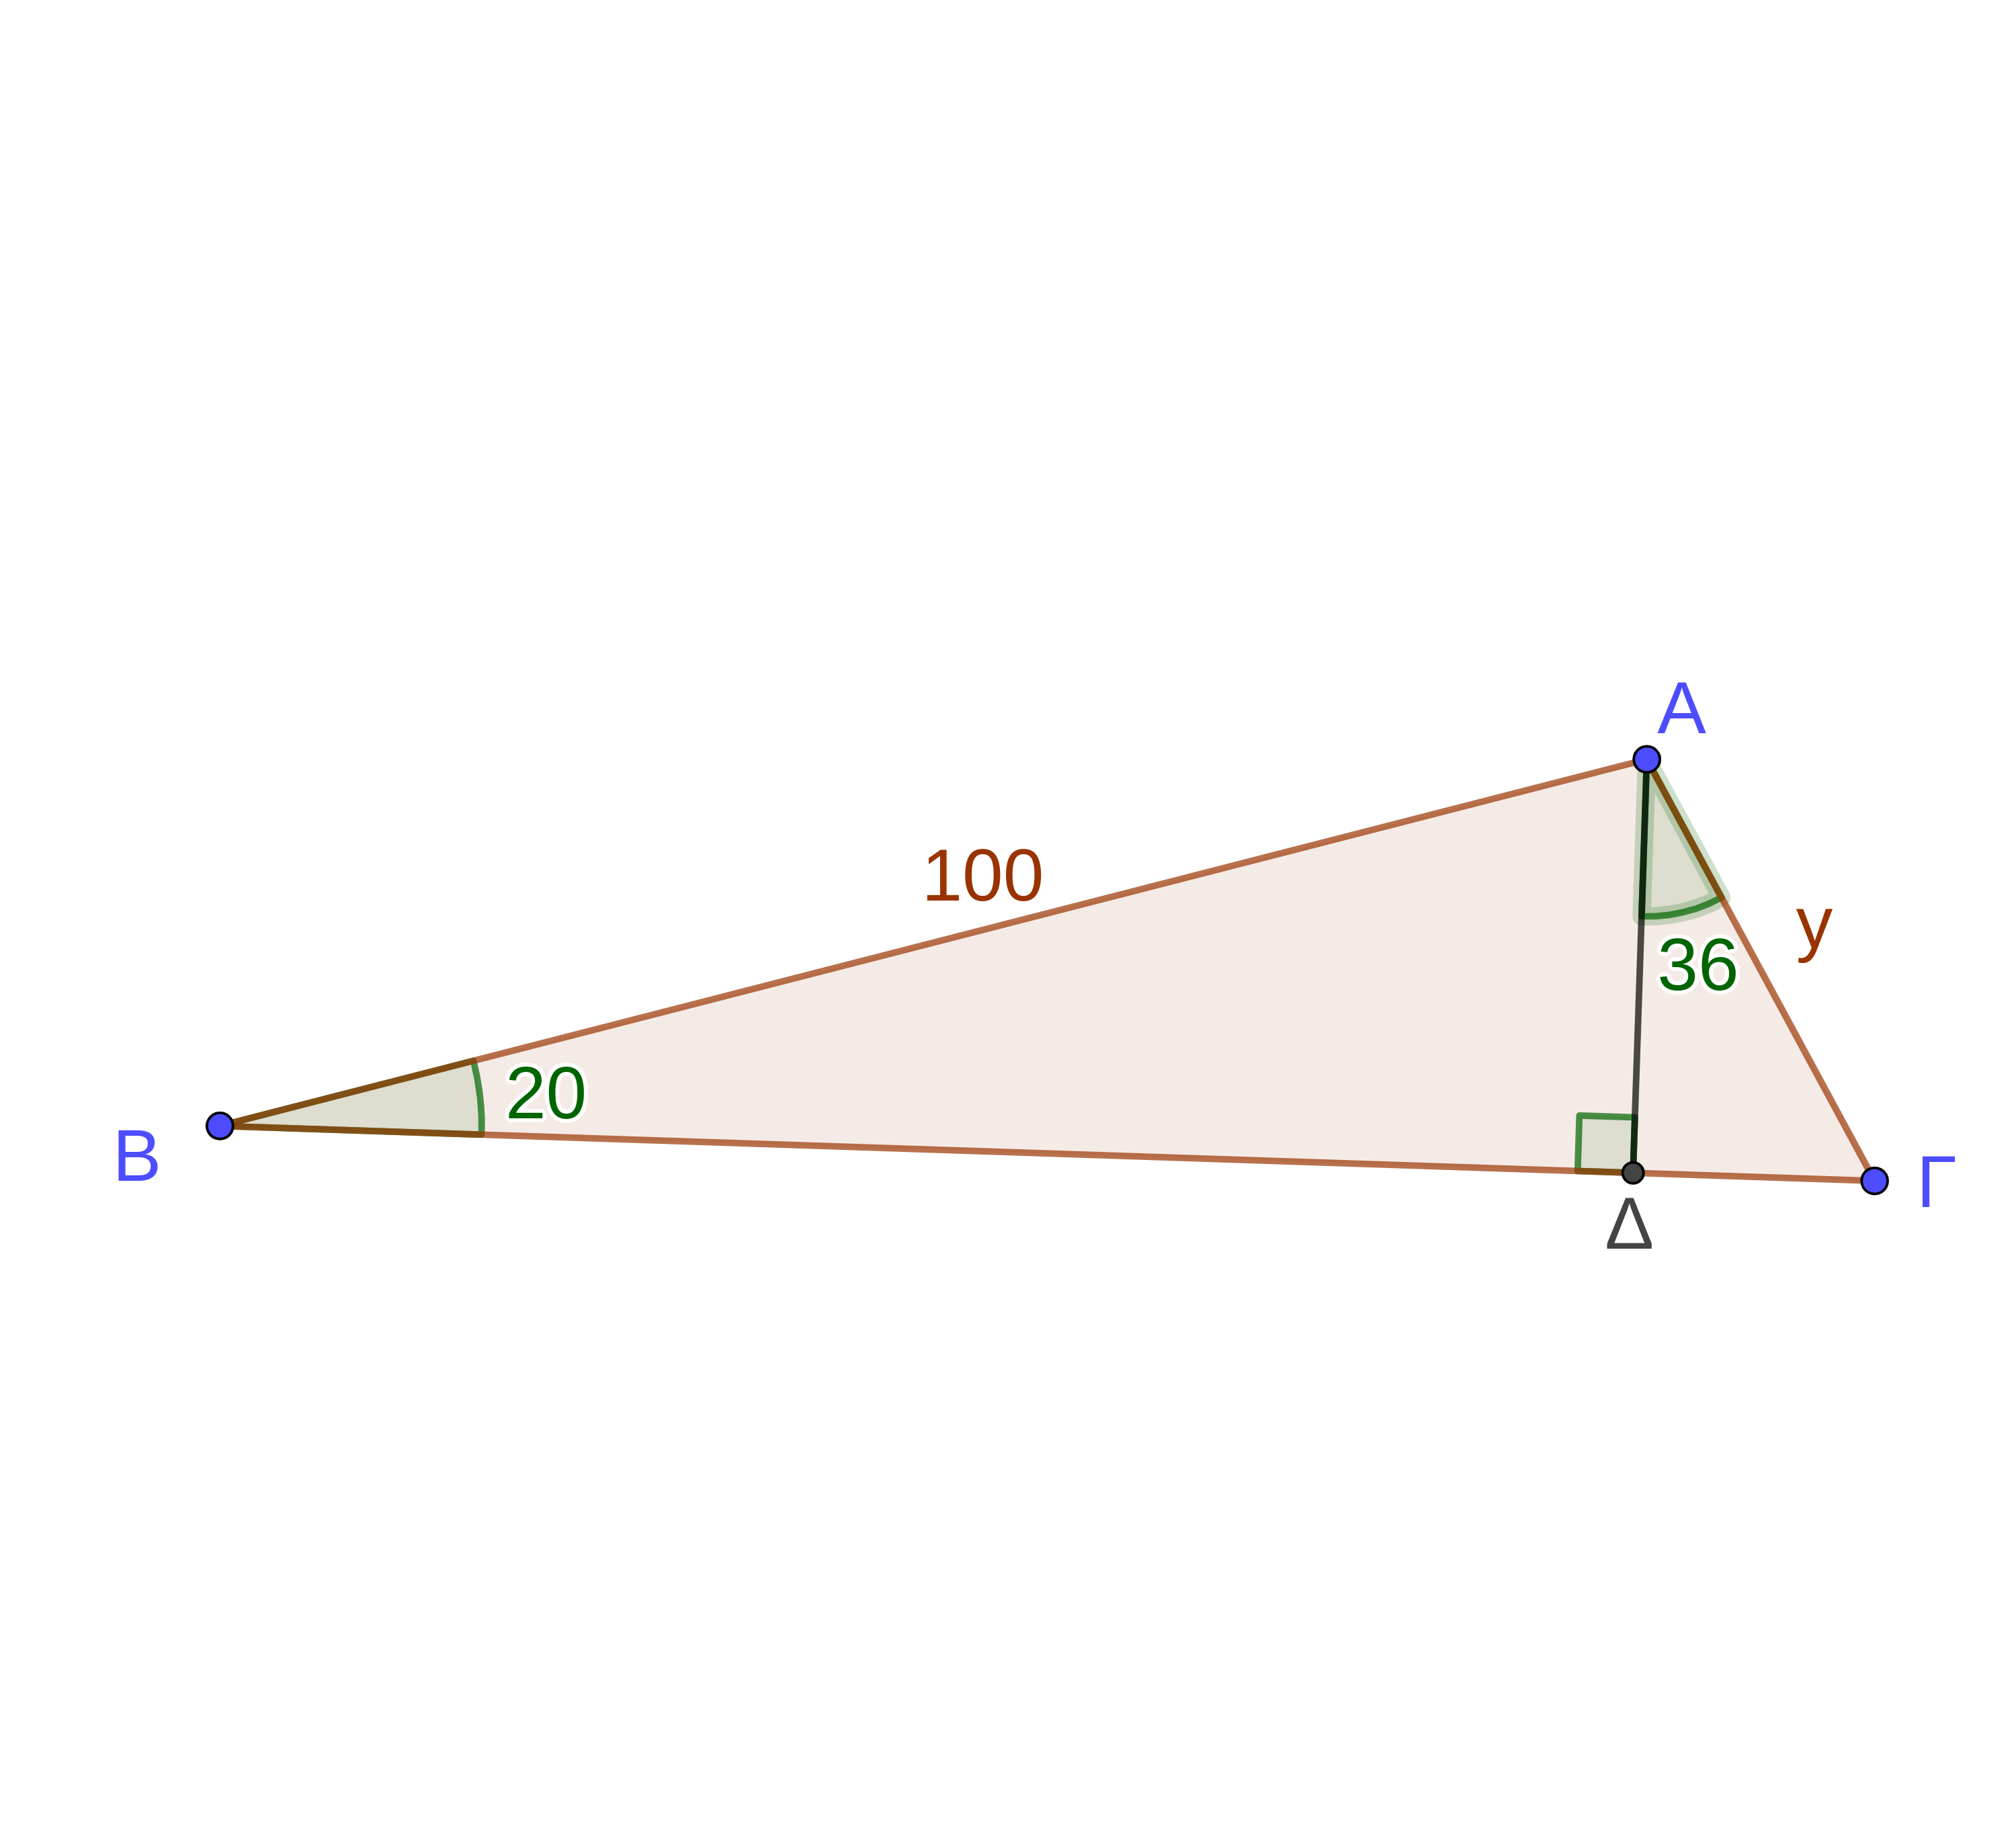
\includegraphics[width=0.8\textwidth]{"./images/3.1.1_3.png"}
\end{askisi}

\begin{askisi}
  Μια επίκεντρη γωνία $ω$ βαίνει σε τόξο μήκους $S=20cm$. Να εκφράσετε τη γωνία $ω$ σε ακτίνια, αν η ακτίνα του κύκλου είναι $ρ=5cm$.
\end{askisi}

\begin{askisi}
  Να εκφράσετε τη γωνία
  \begin{itemize}
    \item<1-> $120^{\circ}$ σε rad
    \item<2-> $\dfrac{3π}{4}$ rad σε μοίρες
  \end{itemize}
\end{askisi}

\begin{askisi}
  Να υπολογίσετε την τιμή των παραστάσεων:
  \begin{itemize}
    \item<1-> $Α=ημ90^{\circ}-συν60^{\circ}+σφ45^{\circ}-συν180^{\circ}$
    \item<2-> $Β=ημ\dfrac{π}{6}-συν^2\dfrac{π}{6}-εφ\dfrac{π}{4}\cdot σφ\dfrac{π}{2}$
  \end{itemize}
\end{askisi}

\begin{askisi}
  Να υπολογίσετε τους τριγωνομετρικούς αριθμούς των γωνιών
  \begin{itemize}
    \item<1-> $765^{\circ}$
    \item<2-> $\dfrac{5π}{2}$ rad
    \item<3-> $\dfrac{49π}{6}$ rad
  \end{itemize}
\end{askisi}

\begin{askisi}
  Να βρείτε το πρόσημο των παραστάσεων:
  \begin{itemize}
    \item<1-> $Α=ημ100^{\circ}-συν200^{\circ}-εφ1000^{\circ}$
    \item<2-> $Β=ημ1-συν2$
    \item<3-> $Γ=συν3 \cdot εφ5$
  \end{itemize}
\end{askisi}

\begin{askisi}
  Να βρείτε το πρόσημο των παραστάσεων:
  \begin{itemize}
    \item<1-> $Α=συν^2x-συνx-εφx$, $x\in (\dfrac{π}{2},π]$
    \item<2-> $Β=συν\dfrac{x}{2}+ημ2x-συν3x$, $\dfrac{π}{4}<x<\dfrac{π}{2}$
  \end{itemize}
\end{askisi}

\begin{askisi}
  Να βρείτε μεταξύ ποιων αριθμών βρίσκονται οι τιμές των παραστάσεων:
  \begin{itemize}
    \item<1-> $Α=2-5ημx$
    \item<2-> $Β=3-2συν^2x$
    \item<3-> $Γ=\dfrac{1}{5-2ημx}$
  \end{itemize}
\end{askisi}

\section{}
\begin{frame}
  Στο moodle θα βρείτε τις ασκήσεις που πρέπει να κάνετε, όπως και αυτή τη παρουσίαση
\end{frame}

% \appendix
% \section{Λύσεις Ασκήσεων}
% \begin{frame}
%  \tableofcontents
% \end{frame}

\end{document}
